% !TEX encoding = UTF-8 Unicode
\documentclass[a4paper]{report}

\usepackage[utf8]{inputenc}
\usepackage[francais]{babel}
\usepackage[nonewpage]{imakeidx}
\usepackage{hyperref}
\usepackage{enumitem}
\usepackage{graphicx}
\usepackage{array}
\usepackage{float}
\usepackage{fancyhdr}

% Glossaire:
\usepackage[acronym,toc,nopostdot, nonumberlist]{glossaries}
% !TEX encoding = UTF-8 Unicode
% Glossaire
\newglossaryentry{joueur}
{
    name=joueur,
    description={Personnage fictif du jeux pouvant faire partie d'une équipe et jouant au quiditch.}
}
\newglossaryentry{equipe}
{
    name=équipe,
    description={Elle est composée de 7 \glspl{joueur} (un gardien, un attrapeur, deux batteurs et trois poursuive).}
}
\newglossaryentry{manager}
{
    name=manager,
    description={\Gls{utilisateur} du programme, il possède un \gls{club} et dois faire en sorte que celui-ci gagne de l'argent.}
}
\newglossaryentry{club}
{
    name=club,
    description={Infrastructure contenant une \gls{equipe} et des installations (stade, infirmerie,\ldots).}
}

\newglossaryentry{utilisateur}
{
    name=utilisateur,
    description={Personnage réel. C'est la personne qui joue au Quiditch manager.\\
    Elle est appelée en jeu \gls{manager}}
}

\newglossaryentry{enchere}
{
    name=enchère,
    description={Système permettant l'achat de \glspl{joueur}}
}
\newglossaryentry{serveur}
{
    name=serveur,
    description={Programme étant toujours en marche et connecté à internet et qui réceptionne les connections des \glspl{client}. Il a les données de tous les \glspl{utilisateur}.}
}
\newglossaryentry{client}
{
    name=client,
    description={Programme que l'\gls{utilisateur} lance pour se connecter au \gls{serveur}. Il permet à l'\gls{utilisateur} de jouer et peut être soit en ligne de commande, soit en mode graphique.}
}
\newglossaryentry{participant}
{
    name=participant,
    description={Nom donné à l'\gls{utilisateur} lors d'un tournoi.}
}


% Acronymes

\makeglossaries
\setglossarysection{section}
\deftranslation{Glossary}{Glossaire}
\renewcommand*{\glossaryname}{Glossaire}
\DeclareRobustCommand{\gloss}[1]{\it{#1}\index{\glslabel}}
\renewcommand{\glsdisplay}[4]{\gloss{#1#4}}
\renewcommand{\glsdisplayfirst}[4]{\gloss{#1#4}}



\makeindex
\indexsetup{level=\chapter}
\setcounter{secnumdepth}{4}

\title{Quidditch Manager 2014 : \\Software requirements document\\ 
\includegraphics[width=\textwidth]{logo.png}}
\author{Bruno Rocha Pereira \and Romain Fontaine \and Nikita Marchant}
\date{\today}

\begin{document}
\fancypagestyle{empty}{
  \fancyhf{}
  \fancyhead[L]{
\includegraphics[scale=0.5]{logoulb.jpg}}
}
\maketitle
\tableofcontents
\clearpage


\chapter{Introduction}
\section{But du projet}
Le but du projet d'année en BA2 en sciences informatiques est le développement d'une application de jeu multi-joueur en ligne.
Il consiste en l'implémentation d'un jeu de Quidditch, sport tiré de la saga Harry Potter de J.K.Rowling.


Le Quidditch est un sport pratiqué par deux \glspl{equipe} de 7 \glspl{joueur} évoluant à l'aide de leur balais sur un terrain de forme ovale. Le but de ces 2 \glspl{equipe} est de marquer le plus de points possible en marquant à l'aide du souaffle dans un des 3 buts adverses et d'attraper le vif d'or\footnote{Pour plus d'informations, se référer au livre J. K. Rowling : "Le Quidditch à travers les âges", Gallimard, 2001.}, ce qui signe la fin du match. 


Notre application sera un jeu de gestion et stratégie en ligne, se jouant individuellement pendant la gestion et au tour par tour à 2 joueurs lors des matchs. L'\gls{utilisateur} est le \gls{manager} d'un \gls{club} de Quidditch et son but est de faire progresser son \gls{club} vers le succès. Pour ce faire, il devra gérer tous les aspects du \gls{club}, tant au niveau sportif que financier. Il aura à sa disposition différentes installation pour entraîner ses \glspl{joueur} ou gagner de l'argent. Il pourra améliorer les différentes installation de son \gls{club} à l'aide d'argent.

Cet argent sera récolté lors des matchs et grâce aux revenus générés par les différents magasins du \gls{club}. La saison de Quidditch se déroule sous la forme d'un championnat, durant lequel tous les \glspl{utilisateur} inscrits s'affrontent entre eux au cours de matches. Les matches seront planifiés dans un calendrier qu'il faudra respecter sous peine de sanction. Un match se joue au tour part tour, mais les deux \glspl{utilisateur} jouent simultanément, le \gls{serveur} résolvant les conflits à la fin de chaque tour. Il y a donc une notion importante d'anticipation dans la maîtrise de ce jeu.

En ce qui concerne la gestion du \gls{club}, l'\gls{utilisateur} aura la possibilité de recruter de nouveaux \glspl{joueur} de Quidditch pour renforcer son \gls{equipe} via un système d'\glspl{enchere}, il pourra aussi développer différentes infrastructures et services comme son stade, son infirmerie, son terrain d'entraînement, son fanshop etc.

% glossaire

\printglossary[numberedsection]
\section{Historique}
\begin{description}
    \item[0.1] (05/12/13) : Création du document - Equipe
    \item[0.2] (10/12/13) : Premier jet de chaque partie - Equipe
    \item[0.3] (11/12/13) : Création des diagrammes UML - Bruno, Tsotne
    \item[0.4] (11/12/13) : Amélioration des différents requirements - Nikita
    \item[0.5] (12/12/13) : Ajout du glossaire - Romain
    \item[0.6] (14/12/13) : Ajout du use case d'authentification et ajout des descriptions des use case - Tsotne
    \item[0.7] (15/12/13) : Finalisation des use case - Tsotne
    \item[0.8] (15/12/13) : Ajout de l'index et de la table des figures - Nikita
    \item[0.9] (19/12/13) : Corrections et ajout des diagrammes au document - Bruno, Tsotne
    \item[1.0] (20/12/13) : \textbf{Délivrable pour la phase 1 - Equipe}

    \item[1.1] (16/02/14) : Correction de fautes d'orthographes et remplissage de l'historique - Bruno
    \item[1.2] (18/02/14) : Ajout et correction de diagrammes de classe - Bruno
    \item[1.3] (20/02/14) : Modification du type de document et ajout des chapitres - Romain
    \item[1.4] (20/02/14) : Ajout du justificatif de choix de librairie graphique - Bruno
    \item[1.5] (21/02/14) : Ajout des diagrammes d'activité - Bruno
    \item[1.6] (21/02/14) : Finalisation de la justification de choix de librairie graphique - Bruno
    \item[1.7] (21/02/14) : Ajout des diagrammes de composants - Cédric
    \item[2.0] (21/02/14) : \textbf{Délivrable pour la partie 2 - Equipe}

    \item[2.1] (12/03/14) : Correction du diagramme de classe général - Bruno
    \item[2.2] (13/03/14) : Ajout du paragraphe "Idées de fonctionnalités" - Bruno
    \item[3.0] (/03/14) : \textbf{Délivrable pour la partie 3 - Equipe}
    
    \item[3.1] (31/03/14) : Modification de la page de garde - Bruno
    \item[3.2] (01/04/14) : Correction des component diagrams - Bruno
    \item[3.3] (04/04/14) : Ajout des nouveaux diagrammes de classe - Romain
    \item[3.4] (04/04/14) : Ajout des nouveaux use-case diagrams - Bruno
    \item[3.5] (04/04/14) : Ajout du sequence diagram - Nikita
    \item[3.6] (04/04/14) : Ré-organisation du document et suppression des parties obsolètes ou non implémentées - Nikita
	\item[3.6] (07/04/14) : Corrections orthographiques - Nikita
	\item[3.7] (07/04/14) : Ajout de nouveaux diagrammes d'activité - Nikita
	\item[3.8] (07/04/14) : Ajout de diagrammes de classe - Romain
	\item[3.9] (07/04/14) : Ajout de diagrammes de séquence - Nikita
	\item[3.10] (07/04/14) : Correction de la mise en page - Nikita
    
    \item[4.0] (07/04/14) : \textbf{Délivrable pour la partie 4 - Equipe}
    


\end{description}


\chapter{Besoins d'utilisation}
\section{Exigences fonctionnelles}

\subsection{Gestion des utilisateurs}

\begin{figure}[H]
    \begin{center}
        \includegraphics[width=\textwidth]{uml/useCaseDiadrams/ConnectionUCD.eps}
        \caption{\label{diag-use-inscription} Système d'identification}
    \end{center}
\end{figure}

\subsubsection{Inscription}

\begin{description}
    \item[Cas général  :] L'\gls{utilisateur} doit pouvoir s'inscrire (s'enregistrer) sur le \gls{serveur} avec un nom d'\gls{utilisateur} unique et un mot de passe.
    \item[Pré Condition  :] L'\gls{utilisateur} n'est pas déjà connecté
    \item[Post Condition :] L'\gls{utilisateur} aura fait une demande d'inscription.
    \item[Cas Exceptionnel :] L'inscription échouera et l'\gls{utilisateur} sera invité à recommencer si le nom de compte est déjà enregistré sur le \gls{serveur}.
\end{description}

\subsubsection{Connection}
\begin{description}
    \item[Cas général :] L'\gls{utilisateur} doit pouvoir se connecter en s'authentifiant auprès du \gls{serveur} avec son nom d'\gls{utilisateur} et son mot de passe.
    \item[Pré Condition  :] L'\gls{utilisateur} n'est pas déjà connecté
    \item[Post Condition :] L'\gls{utilisateur} aura fait une demande de connexion.
    \item[Cas Exceptionnel :] L'authentification échouera et l'\gls{utilisateur} sera invité à recommencer si le mot de passe ne correspond pas au nom d'\gls{utilisateur}, ou cet \gls{utilisateur} n'existe sur le \gls{serveur}.
\end{description}

\subsection{Gestion du club}


\begin{figure}[H]
    \begin{center}
        \includegraphics[width=\textwidth]{uml/useCaseDiadrams/MenuUCD.eps}
        \caption{Menu principal}
    \end{center}
\end{figure}

\subsubsection{Gestion des infrastructures}
\begin{figure}[H]
    \begin{center}
        \includegraphics[width=\textwidth]{uml/useCaseDiadrams/InfrastructuresUCD.eps}
        \caption{Gestion des infrastructures}
    \end{center}
\end{figure}


\subsection{Jouer à un match}
\subsubsection{Jouer un tour}
\begin{description}
    \item[Cas général :] L'\gls{utilisateur} doit pouvoir jouer un tour lors d'un match, c'est à dire déplacer ses \glspl{joueur} et/ou effectuer des actions.
    \item[Pré Condition  :] L'\gls{utilisateur} doit être entrain de jouer à un match.
    \item[Post Condition :] L'\gls{utilisateur} aura joué son mouvement.
    \item[Cas Exceptionnel :] La perte de connexion avec un \gls{utilisateur} maintenue, durant un certain timeout, entraînera son remplacement pour ce match par une IA fournie par le système. Le match continuera sans changement.
\end{description}
\subsubsection{Déclarer forfait}
\begin{description}
    \item[Cas général :] L'\gls{utilisateur} peut déclarer forfait durant un match (il sera considéré comme perdant).
    \item[Pré Condition  :] L'\gls{utilisateur} doit être entrain de jouer à un match.
    \item[Post Condition :] L'\gls{utilisateur} sera déclaré comme perdant.
\end{description}

\subsection{Gestion des défis}
\subsubsection{Défier un utilisateur}
\begin{description}
    \item[Cas général :] L'\gls{utilisateur} peut défier un autre utilisateur au choix parmi un liste d'utilisateurs connectés au serveur
    \item[Pré Condition  :] L'\gls{utilisateur} ainsi que l'autre utilisateur doivent être connectés et ne pas jouer de match,
    \item[Post Condition :] L'\gls{utilisateur} l'utilisateur adverse reçoit une notification de défi
\end{description}

\subsubsection{Accepter un défi}
\begin{description}
    \item[Cas général :] L'\gls{utilisateur} reçoit une notification lui demandant d'accepter un défi et il l'accepte
    \item[Pré Condition  :] L'\gls{utilisateur} doit avoir été défié par un autre utilisateur
    \item[Post Condition :] L'\gls{utilisateur} un match est créé et les deux utilisateurs commencent à jouer
\end{description}

\subsubsection{Refuser un défi}
\begin{description}
    \item[Cas général :] L'\gls{utilisateur} reçoit une notification lui demandant d'accepter un défi et il le refuse
    \item[Pré Condition  :] L'\gls{utilisateur} doit avoir été défié par un autre utilisateur
    \item[Post Condition :] Les deux utilisateurs repassent en phase de management normale.
\end{description}

% fin de "Exigences fonctionnelles"
%%%%%%%%%%%%%%%%%%%%%%%%%%%%%%%%%%%

\section{Exigences non fonctionnelles}
\begin{itemize}
    \item La machine hébergeant le \gls{client} ainsi que le \gls{serveur} doivent être en mesure de communiquer en permanence via un réseau capable de transporter des paquets \textbf{TCP/IP}
    \item Le réseau décrit ci-dessus doit pourvoir une latence raisonnablement faible (c'est à dire moins de 500ms pour un aller retour) et disposer du port 9000/tcp ouvert en sortie pour le serveur et en entrée pour le client.
    \item Les machines exécutant le \gls{client} doivent être équipées d'un écran, d'un clavier et d'une souris et être capables d'afficher des images en mode graphique ainsi qu'au minimum 80 caractères de large en mode console. Elles devront aussi avoir au minimum disposer de 128MB de mémoire vive ainsi que 128MB d'espace disque.
\end{itemize}

% fin de "Exigences non fonctionnelles"
%%%%%%%%%%%%%%%%%%%%%%%%%%%%%%%%%%%%%%%

\section{Exigences de domaine}
\begin{itemize}
    \item Le jeu doit être multi-joueur, les différents \glspl{utilisateur} connectés sur un même \gls{serveur} doivent pourvoir interagir entre eux.
    \item Le monde doit être persistent : il doit continuer d'évoluer, même en l'absence d'un ou plusieurs \glspl{utilisateur}.
    \item Une \gls{equipe} de Quidditch doit comporter 7 \glspl{joueur} au maximum, sans compter les remplaçants.
    \item Un \gls{joueur} blessé/mort ne peut être remplacé en plein match.
    \item Un match nécessite trois balles : Un souaffle, deux cognards et un vif d'or. Le terrain doit comporter deux buts, fait chacun de trois anneaux, et placé aux deux extrémités.
    \item Pour participer à un match, chaque \gls{joueur} doit posséder un balai.
    \item Le match ne prend fin que si le vif d'or est attrapé ou que l'une des deux \glspl{equipe} abandonne.

\end{itemize}

% fin de "Exigences de domaine"
%%%%%%%%%%%%%%%%%%%%%%%%%%%%%%%%%%%%%%%

\chapter{Besoin du système}
\section{Exigences fonctionnelles}

\subsection{Identification}
\subsubsection{Enregistrer une inscription}
\begin{description}
    \item[Cas général :] Le système doit être capable d'enregistrer un nom de compte unique associé à un mot de passe dans un fichier, ainsi que de vérifier que le nom de compte fourni est unique.
    \item[Pré Condition  :] Un \gls{utilisateur} effectuant une demande d'inscription.
    \item[Post Condition :] Le nom de compte sera enregistré sur le \gls{serveur}. L'\gls{utilisateur} sera donc inscrit.
    \item[Cas Exceptionnel :] L'enregistrement échouera si le nom de compte est déjà enregistré sur le fichier.
\end{description}

\subsubsection{Authentifier un utilisateur}
\begin{description}
    \item[Cas général :] Le système doit être capable d'authentifier un \gls{utilisateur} demandant de se connecter en vérifiant que le nom de compte fourni lors de la connexion est présente dans le fichier du \gls{serveur} et est bien associé au mot de passe fourni.
    \item[Pré Condition  :] Un \gls{utilisateur} effectuant une demande de connexion.
    \item[Post Condition :] L'\gls{utilisateur} sera connecté.
    \item[Cas Exceptionnel :] L'authentification échouera si le nom de compte fourni n'est pas enregistré sur le \gls{serveur}, ou s'il est associé à un autre mot de passe que le mot de passe fourni.
\end{description}

\subsection{Interface}
\subsubsection{Fournir une interface}
\begin{description}
    \item[Cas général :] Le système doit fournir à l'\gls{utilisateur} une interface jeu simple, complète et interactive, graphique et en console pour les deux phases de jeu.
\end{description}

\subsubsection{Représenter phase management}
\begin{description}
    \item[Cas général :] Le système doit fournir à l'\gls{utilisateur} une représentation du \gls{club} (phase management), comprenant une vue d'ensemble sur son argent, ses rentrées, ses \glspl{joueur}, ses infrastructures et les améliorations possibles.
\end{description}

\subsubsection{Représenter un match}
\begin{description}
    \item[Cas général :] Le système doit fournir à l'\gls{utilisateur} une représentation du terrain ovale (pendant la phase de match), sous forme de cases hexagonales.
\end{description}


\subsection{Divers}
\subsubsection{Sauvegarder}
\begin{description}
    \item[Cas général :] Le système doit sauvegarder tout changement effectué au \gls{club} durant la phase de management ainsi qu'après une partie.
    \item[Pré Condition  :] Une modification du \gls{club} en phase management, ou une fin de match.
    \item[Post Condition :] Les changements apportés au \glspl{club} et au \gls{serveur} seront sauvegardés.
    \item[Cas Exceptionnel :] Aucun changement du aux match en cours ne sera sauvegardé si \gls{serveur} plante.
\end{description}


\section{Exigences non fonctionnelles}
\label{enf}
\begin{itemize}
    \item Le \gls{client} et le \gls{serveur} doivent être écrits en \textbf{C++} et seront compilés à l'aide de \textbf{gcc 4.8}
    \item Le \gls{client} et le \gls{serveur} doivent être portables et pouvoir fonctionner sur un système \textbf{UNIX} et une architecture x86
    \item La machine exécutant le \gls{serveur} doit être capable de gérer une connexion ouverte constamment vers chaque \gls{client} ainsi que de stocker l'entièreté des données du jeu en mémoire disque ainsi qu'une grande majorité en mémoire vive.
\end{itemize}


\section{Design et fonctionnement}
\subsection{Diagrammes de classe}

\begin{figure}[H]
    \makebox[\linewidth]{
        \includegraphics[height=430pt]{uml/classDiagrams/manager.eps}
    }
    \caption{Diagramme de classe : Manager}
\end{figure}

\begin{figure}[H]
    \makebox[\linewidth]{
        \includegraphics[width=430pt]{uml/classDiagrams/match.eps}
    }
    \caption{Diagramme de classe : Match}
\end{figure}

\begin{figure}[H]
    \makebox[\linewidth]{
        \includegraphics[width=270pt]{uml/classDiagrams/userHandler.eps}
    }
    \caption{Diagramme de classe : UserHandler}
\end{figure}

\begin{figure}[H]
    \makebox[\linewidth]{
        \includegraphics[height=200pt]{uml/classDiagrams/socket.eps}
    }
    \caption{Diagramme de classe : Socket}
\end{figure}

\begin{figure}[H]
    \makebox[\linewidth]{
        \includegraphics[width=430pt]{uml/classDiagrams/json.eps}
    }
    \caption{Diagramme de classe : Json}
\end{figure}

\begin{figure}[H]
    \makebox[\linewidth]{
        \includegraphics[width=270pt]{uml/classDiagrams/mainWindow.eps}
    }
    \caption{Diagramme de classe : mainWindow}
\end{figure}

\begin{figure}[H]
    \makebox[\linewidth]{
        \includegraphics[width=220pt]{uml/classDiagrams/serverHandler.eps}
    }
    \caption{Diagramme de classe : ServerHandler}
\end{figure}



\subsection{Diagrammes d'activité}

\begin{figure}[H]
    %\vspace*{-3cm}
    \makebox[\linewidth]{
        \includegraphics[width=430pt]{uml/activityDiagrams/generalActivityDiagram.eps}
    }
    \caption{Diagramme d'activité}
\end{figure}

\begin{figure}[H]
    %\vspace*{-3cm}
    \makebox[\linewidth]{
        \includegraphics[width=410pt]{uml/activityDiagrams/challengeActivityDiagram.eps}
    }
    \caption{\label{3} Diagramme d'activité représentant le lancement de défis}
\end{figure}

\begin{figure}[H]
    %\vspace*{-3cm}
    \makebox[\linewidth]{
        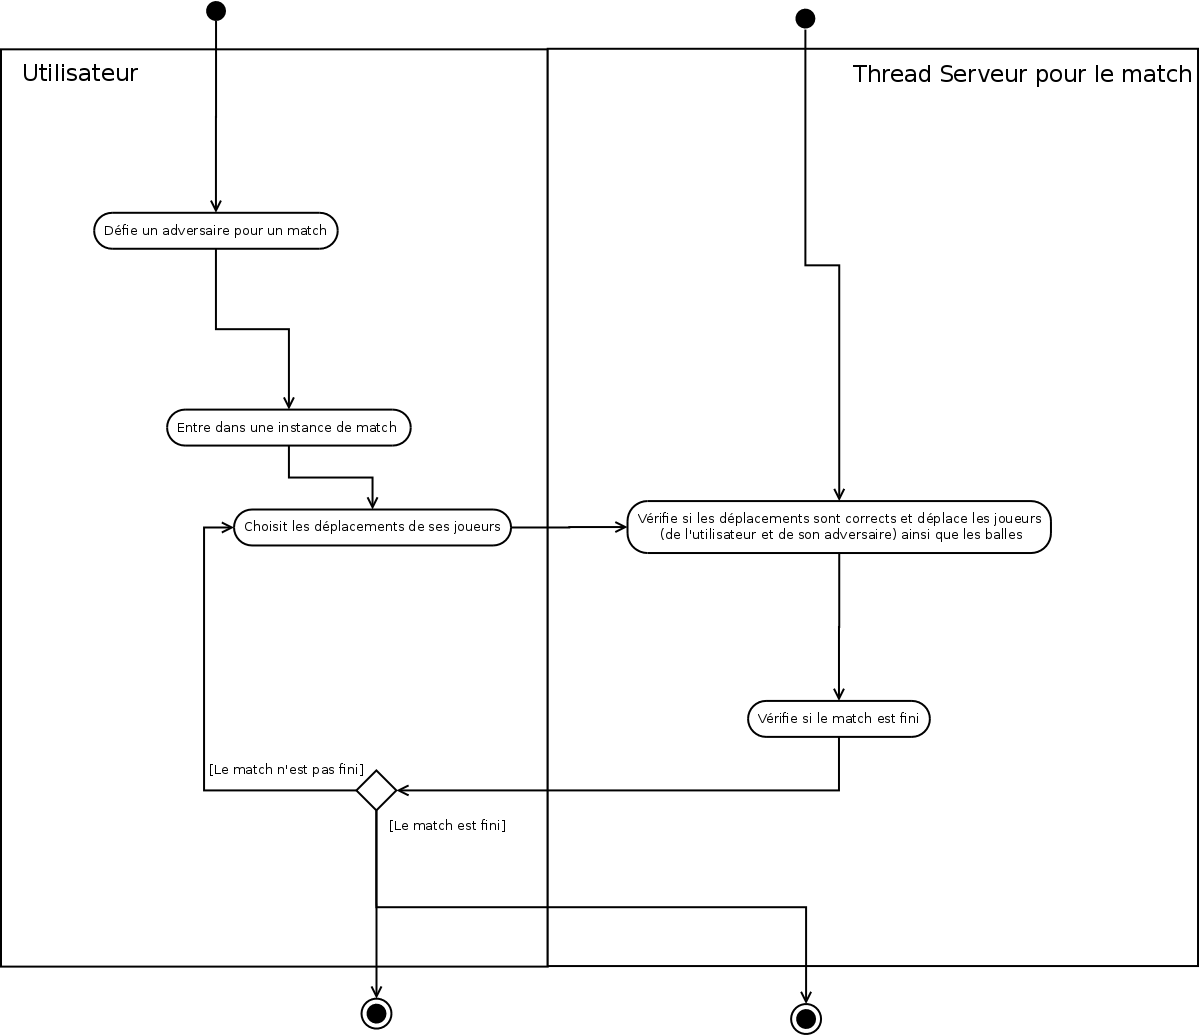
\includegraphics[width=380pt]{uml/activityDiagrams/matchActivityDiagram.eps}
    }
    \caption{\label{3} Diagramme d'activité représentant le déroulement d'un match}
\end{figure}

%DIAGRAMES DE COMPOSANTS
\subsection{Diagrammes de composants}

\begin{figure}[H]
    \makebox[\linewidth]{
        \includegraphics[width=430pt]{uml/inclusions.eps}
    }
    \caption{Diagramme de composants}
\end{figure}

\subsection{Diagrammes de séquence}

\begin{figure}[H]
    \makebox[\linewidth]{
        \includegraphics[width=430pt]{uml/sequence/loginseq.eps}
    }
    \caption{Diagramme de séquence : connexion}
\end{figure}


\begin{figure}[H]
    \makebox[\linewidth]{
        \includegraphics[width=440pt]{uml/sequence/matchseq.eps}
    }
    \caption{Diagramme de séquence : enregistrement}
\end{figure}

\begin{figure}[H]
    \makebox[\linewidth]{
        \includegraphics[width=430pt]{uml/sequence/challengeseq.eps}
    }
    \caption{Diagramme de séquence : défi}
\end{figure}


\begin{figure}[H]
    \makebox[\linewidth]{
        \includegraphics[width=430pt]{uml/sequence/matchseq.eps}
    }
    \caption{Diagramme de séquence : match}
\end{figure}




\chapter{Justification de la bibliothèque graphique}
\section{Qt}
\subsection{Avantages}
\begin{itemize}
    \item Qt est une librairie complète et possède une documentation énorme. De ce fait, il sera facile de trouver réponse à nos questions.
    \item Qt est une librairie utilisée depuis 1995 et le projet est toujours actif et maintenu par une grande société (Nokia), on peut donc la considérer comme stable.
    \item Qt est écrit en C++ et donc nativement adapté pour ce langage.
    \item Qt est OpenSource (sous license GNU LGPL).
    \item Qt permet d'utiliser le framework QgraphicsView, facile d'utilisation et complet, permettant de dessiner aisément ce que l'on veut.
    \item On peut utiliser Qt Creator pour cette librairie graphique, IDE fournissant une auto-complétion pour tous les modules de Qt et possédant une aide disponible intrinsèque.
\end{itemize}
\subsection{Inconvénients}
\begin{itemize}
    \item Lourd
    \item Possède des packages qui ne nous serviront pas, étant donné que nous ne n'utiliserons que la partie graphique de Qt
\end{itemize}
\section{GTK+}
\subsection{Avantages}
\begin{itemize}
    \item Plus léger
\end{itemize}
\subsection{Inconvénients}
\begin{itemize}
    \item Documentation non complète
    \item Pas d'IDE fourni par l'équipe en charge du projet GTK+
\end{itemize}
\section{Conclusion}
Nous utiliserons donc Qt, de par la présence et la simplicité d'utilisation de son IDE \textit{Qt Creator} et par la richesse de la documentation qui l'accompagne. La stabilité de cette API fut également un élément influençant notre choix.

\chapter{Idées d'ajout de fonctionnalités}
\section{A finir}
\begin{itemize}
    \item Les \glspl{enchere}
    \item Un système d'admin
    \item Gestion d'équipes
    \item Points d'actions
    \item Sponsors
\end{itemize}
\section {Fonctionnalités supplémentaires}
\begin{itemize}
    \item Équipes nationales
    \item Événements aléatoires
    \item Boîte à message
    \item Statistiques
\end{itemize}



\printindex
\listoffigures
%\listoftables

\end{document}
